\chapter{Background}\label{chap:bg}
Using knowledge in a WSN is related to existing research into sensor networks that utilise context-awareness in order to improve their effectiveness or adapt their sampling rate. An example of a context-aware sensor is an accelerometer attached to a node that is able to determine what the readings of the accelerometer indicate. For example, a smart phone with an accelerometer may use context-awareness to determine if the user is running, walking or going upstairs. Some of these actions may be more important than others and, thus, they can be prioritised. However, researching context-aware WSNs alone would limit our knowledge of WSNs in general and affect decisions we make when designing our own architecture. There is research that is valuable for all types of sensor network, such as: hardware design, routing protocol, tranmission medium choice or middleware used.

This chapter is split into the following sections. Section \ref{bg:wsni} outlines the issues surrounding WSN design and deployment. 
Section \ref{bg:rp} details relevant existing routing protocols for sensor networks. Section \ref{bg:sm} highlights commonly-used sensor middleware. Section \ref{bg:bsn} shows some examples of existing WSNs that are related to our motivating scenario. Section \ref{bg:lgk} introduces research into local and global knowledge and Section \ref{bg:rsn} shows related work into WSNs that utilise knowledge or context-awareness.

\section{Wireless Sensor Network Issues} \label{bg:wsni}

WSNs have been used in a number of domains, for a range of different purposes, from habitat monitoring \cite{Szewczyk2004a} to military purposes \cite{Pizzocaro} and healthcare \cite{Otto2006}. While these applications are different, the technology behind each is very similar. Each requires the use of nodes with sensors attached and each node requires a power source and storage devices.

According to \cite{Akyildiz2002}, there are at least eight factors that affect the design of sensor networks, but we focus on a subset that are the most relevant to our research problem. Those we have given less consideration to are: production costs, scalability and topology. While these are important, productions costs rae not a concern for us in the research stages and scalability has been considered when researching existing networks to follow existing \textit{gold standard} practices. We have considered the following points in greater detail:

\subsection{Fault Tolerance}
	WSNs typically contain a large number of nodes and any node can fail for various reasons, from a lack of power, filling its storage capacity, to factors in the environment causing the hardware to fail. While the hardware architecture of sensor nodes is typically similar, the variation between each deployment means that the device itself must be adapted to its environment. For example, \cite{Mainwaring2002} used a custom protective casing for their nodes so that they were able to survive being in the open while ensuring that the transmission range was not affected.


\subsection{Hardware Constraints}
	A sensor node typically consists of: a platform that contains the memory and processing power,  a sensor (or sensors) and a transceiver that uses a wireless standard, such as Wi-Fi or Zigbee. Cost and size are the most significant considerations when designing a WSN. According to \cite{Intanagonwiwat2000}, the expectation of a sensor node is a matchbox-sized form factor. However, ten years ago, there was much research focussed on \textit{smart dust} \cite{Kahn}. Smart dust is small, inexpensive, disposable nodes that can transmit until their power reserve is depleted, \cite{Akyildiz2002a} highlights that it is a requirement for the nodes to cost less than USD10. In \cite{Corke2010a}, a decade on from the first WSN papers, smart dust has not been realised and the focus has instead been on larger, more powerful nodes that have reduced in cost and grown in power. 

	The Gartner Hype Cycle for 2013 \cite{gartner2013} shows that smart dust is still in early innovation stages and may not be fully commercialised for another ten years. To counter this, research has been focussed on using software solutions to maximise the battery life in these more powerful, more expensive nodes, accompanied by the use of renewable energy sources.

\subsection{Energy Constraints}
	 Commonly, sensor nodes do not have access to a constant power supply and must run on a battery that is, generally, a similar size to the node. Larger batteries must be contained in a separate battery and this makes nodes less compact and their deployment more difficult. This means that the nodes must be as efficient as possible, knowing when to transmit data and when to sleep. The lifetime of a sensor network is highly dependent on the battery life of each node and, unlike other mobile devices, they cannot typically be recharged \cite{Akyildiz2002}. Much work has been done on power efficient routing protocols, as well as the control of which attached devices are active \cite{Hempstead2005, Schurgers, Segal2010a}. 

	The limited resources on the nodes mean that the sensing devices, and transceivers, attached must consume as little power as possible. Some routing protocols implement turning off wireless radios and scheduling a wakeup across the network \cite{Vaidya2004}, but the cost of turning off a device can waste just as much energy as leaving it on and sampling at a lower rate, if not more \cite{Estrin2001}.

	The use of energy in a node is dependent on how active the sensor(s) are, how much it transmits and receives, the transmission medium used as well as the environment it is in.

\subsection{Transmission Medium}\label{bg:trans}
	Widely used, general purpose transmission media, such as Wi-Fi, are viable solutions in WSNs when a high data rate is required and power is readily available. However, research has shown that Wi-Fi is extremely power-hungry and \cite{Lee2007} shows that Wi-Fi consumes almost 9 times more energy, while transmitting, than other standards, such as Zigbee.
	Bluetooth is a more power-efficient standard that is becoming increasingly popular for sensing devices that are part of the `Quantified Self' movement \cite{Swan2012}, with wearable devices that report measurements, such as heart rate, steps taken and calories burned. With the advent of the new low-power Bluetooh 4.0 , also known as Bluetooth Low Energy (BLE), this standard is supposed to allow months of continuous use on a coin-cell battery \cite{bluetooth2012bluetooth}. However, the range is limited to 100m and, using the same frequency, as Wi-Fi (2.4GHz) means that it is as susceptible to path loss and reduced transfer rates.
	\cite{Zennaro} shows that a 2.4GHz Wi-Fi antenna is capable of transmitting up to 350m, while a considerably lower frequency of 41MHz was able to achieve links of 10km. The use of 2.4GHz frequencies in wet conditions have been shown to reduce the performance by up to 28\% \cite{Markham2010}, while humidity in the air can reduce the performance by up to 78\% \cite{Figueiredo2009}.
	New low-power, low-frequency standards have emerged in recent years and allow for a considerably longer range and increased battery life, at the cost of transmission speeds. Digimesh is an example of this and, while it can achieve 250kb/s using 2.4GHz, it has much slower speeds of 125kbps when using the 900MHz spectrum. However, it does offer a range of, up to, 64Km \cite{Bayat2012}.

\subsection{Environment}
	The environment that a node is deployed in can have a great impact on almost all aspects of a WSN, such as range or the operational lifetime of the node itself. Harsh environments that are not easily accessible make it difficult to place nodes and protected environments may limit where nodes can be placed. 
	In \cite{Martinez2004}, nodes were deployed within glaciers and had to survive extreme temperatures, lasting without human intervention, for months at a time. \cite{Martonosi2003} attached collars to Zebras that had to withstand high speed movement, impact, dust and high temperatures. The deployment of any node requires extensive research as to the environment that it will be deployed in and adjustments must be made to ensure it is able to survive for extended periods without continued maintenance.
	Section \ref{bg:trans} also shows that environment does not simply affect the hardware, but humidity can reduce the transmission range significantly, as well as moisture collecting on wireless antenna can reduce the range for days at a time.

	Limited range in a WSN can be addressed by using `intermediate' nodes - nodes tasked with simply forwarding data from other sensing nodes that would otherwise be out of range - between disconnected sensing nodes. While they do not need to sense the environment directly, they can be vital in ensuring data from all areas of the network are deliverd. In the case of \cite{Martonosi2003}, a car was used to drive near to zebras that had not passed close enough to the base station in order to transmit their data. The car acted as the intermediate node by collecting data from the zebra's collar and relays it back to the base station.

\section{Routing Protocols} \label{bg:rp} 
	Routing protocols specify how nodes in a WSN are organised, as well as how they transmit data throughout the network. In \cite{Akkaya2005}, the more popular routing protocols are surveyed and split into three of the main identified categories: data-centric, hierarchical and location-based. We use the aforementioned categories, as well as flat, to highlight some of the key protocols that are relevant to our work. Flat routing protocols are for WSNs that involve many nodes deployed over a large area, all sending data to a single endpoint. Data-centric is a protocol that focusses on sensed-data, where nodes advertise their contents and query other nodes to fulfill requests made by a user. Location-based protocols use the physical region that nodes are deployed in to request and send data. Hierarchical protocols are for heterogeneous networks that perform more than one task. For example, a network spread of over hundreds of miles could be split into individual networks, or it could follow a hierachical structure where clusters of nodes send data to an endpoint, which then hops across other endpoints in order to reach a final destination.
	The protocols have the task of ensuring that a network is performing at its best, providing the best lifetime and ensuring reliable and consistent delivery of data. This must reduce \textit{flooding}, where nodes send every message to every link, aside from themselves, effectively flooding the network with unnecessary messages, and find a way to deliver data to the endpoint using the most efficient path possible.

\subsection{Flat}
	Initially, this was the most common structure for a WSN, dozens of nodes spread out over a geographical area, with one or more neighbours, sending observations to a single endpoint.

\subsubsection{MCFA} \label{bg:rp:mcfa}
	The Minimum Cost Forwarding Algorithm (MCFA) is a flat routing protocol that works by assigning costs to each node, based on how many hops they are from the endpoint \cite{Ye2001}. 

Each node has a path-estimate of the cost of transmission from itself to the base station. The base station sends out a broadcast message and it is received by all nodes in range. The message contains a cost from the base station (initially zero) while every node has their cost set to infinity. The cost is stored at the node, incremented and sent on to all nodes in range. If the received cost is less than the current cost stored on the node, then the cost (and the neighbour) is updated and passed on.

Each message has a cost associated with it, which is based on the hops it has completed so far. A node that receives the message forwards it only if it's cost matches the sum of the source node's cost (contained within the message) and the message's current cost. This ensures that all messages are sent through the minimum cost path, without storing explicit path information on each node.
% If the cost in the message, plus the link it was received, is less than the current cost. If yes, the estimate is update on both the node and the message; the message is then passed on to other nodes in range. 

	This approach allows for dynamic reconfiguration of the network, as well as a reduced overhead due to not having to maintain a global routing table on each node. The assumption with MCFA, however, is that the direction of routing is always towards a fixed endpoint.

\subsection{Data-centric}
	Data-centric routing protocols are not like traditional WSNs where nodes are given addresses; they use a method that involves the advertising, or querying, of the data that has been sensed and those with the relevant data can respond to the request.

\subsubsection{SPIN}
	Sensor Protocols for Information via Negotation (SPIN) \nomenclature{SPIN}{Sensor Protocols for Information via Negotation} is one of the first data-centric protocols and attempts to address the issue of flooding the network whenever new data is sensed by addressing the data through metadata \cite{Heinzelman1999}. SPIN works on three messages passed between nodes:
	\begin{enumerate}
		\item ADV - A message sent by a node when it has sensed new data, advertising what it has recorded.
		\item REQ - Sent by nodes that received an ADV to request the data.
		\item DATA - Message containing the sensed data.
	\end{enumerate}

When a node has sensed data, it sends an ADV message to all nodes within range. If any of those nodes are interested in the data, then they respond with a REQ message, at which point the DATA message is sent to nodes that responded.

SPIN eliminates the need for a global view of the network topology, as nodes only need to know their single hop neighbours. However, SPIN does not guarantee equal diffusion of data throughout the network as a node may be interested in the data sensed at the other edge of the network, with only nodes that are not interested in between. This would mean that those nodes would not request the data or pass it on.

\subsubsection{SPIN-IT}
	An extension to SPIN, SPIN-IT \nomenclature{SPIN-IT}{Sensor Protocols for Information via Negotation - Image Transfer} uses a slightly different approach to receiving data and is developed solely for the transfer of images \cite{Woodrow2002}, using metadata to fulfill requests.
	
Nodes use the existing message structure of SPIN, but REQ messages are used as queries, sent to all nodes in transmission range. The receiving nodes keep these requests and generate a new REQ message, thus allowing nodes to store temporal paths. When a REQ reaches a node that has the desired data, it responds with a ROUTE-REPLY message. This message is used because images are large and resource-constrained WSNs would have a much shorter lifetime if a lot of unnecessary transmissions were made. The ROUTE-REPLY is used in case multiple nodes, in range of the requesting node, have the data it has requested and it can then choose the optimal route. As each node keeps a history of REQ messages, these can be used to trace the requested data back through the network, to the originating node, without the overhead of maintaining a global routing table.

\subsubsection{COUGAR}
	A slightly different data-centric approach is the proposed COUGAR protocol, viewing the network as a distributed database. Cougar is similar to SPIN because it does not forward data as soon as it is sensed, instead COUGAR uses a query language that abstracts the underlying network structure and uses received queries to generate a plan that utilises in-network processing to provide an answer based on the sensed data stored on all deployed nodes \cite{Yao2002}. 

	For example, in a building monitoring network, a user could query a base station for offices that are unoccupied. The base station then sends that query to all nodes in range and it is then dispersed throughout the network. Nodes that have data that can satisfy the query send back their results and these are combined as they move back through the network to the base station. The user then receives that data, along with the nodes that have provided it.

Within the network, a \textit{leader} is selected and this node is used to aggregate the data from nodes that were able to fulfil all, or some, of the query. At risk of failure, each query should result in a \textit{leader} being dynamically selected and it must have sufficient resources to be able to satisfy the request. This protocol was only proposed, and much of the technical detail has yet to be completed, but the concept of treating the network as a distributed database is a novel idea and this is one of the first protocols to suggest the use of a query language that could be used by people without specific domain knowledge, which, in this case, is technical knowledge of query languages and how the routing protocol works.

\subsection{Hierarchical}
	Hierarchical networks are WSNs that contain nodes of different classes; nodes at the edge of the network are typically clustered into groups and served by a gateway node (also known as a \textit{cluster head}); a node that may not directly sense the environment but acts as an endpoint for a group of nodes \cite{Akkaya2005}. This gateway could be in charge of aggregating the data, processing the data, or simply forwarding it to an endpoint. Clusters of nodes allow the network to be spread out over a wider geographical area and gateway nodes can use a different transmission method to provide long distance links to the base station. Gateway nodes serving a cluster of nodes means that the network can scale easily as well, simply by adding a new cluster to the network.

\subsubsection{TEEN}
	The Threshold sensitive Energy Efficient sensor Network (TEEN) protocol is designed for reactive sensor networks, networks that require instant reactions to changes sensed in their environment \cite{Manjeshwar2001}. TEEN recognises that transmission is the most power hungry action for a node so each node is coded with a hard and soft threshold. The hard threshold is a value that makes nodes transmit the reading to their cluster head. Similarly, the soft threshold is a small change in the value of the sensed attribute that causes further transmissions.

During the initialisation of the network, the base station sends information about the thresholds and sensing attributes to all cluster heads in the network; the cluster heads then forward this on to all nodes in their cluster.  When a node senses data over the hard threshold, it transmits to the cluster and only transmits again when new sensed values are greater than the hard threshold and the difference between the current sensed value and the previous is greater than the soft threshold \cite{Manjeshwar2001}.

Clusters are assigned for a period of time and then new clusters are selected by the base station, at which point new attributes and thresholds are broadcast to all nodes. This kind of protocol allows the network to be dynamic after deployment and allows user input based on the data that has been sensed in the previous cluster times. 

For example, a network could be tasked with sensing humidity in a rainforest but the thresholds have been set such that nodes are transmitting readings that are not of interest. A user can change these thresholds and they will be pushed out to the nodes at the time that the next clusters are chosen, without any need to visit the node or configure them individually.

\subsection{Location-based}
	Instead of using the physical addresses of nodes, or the data they store, location-based protocols are based on the region that nodes are deployed in. Location-based routing relies on the fact that each node is aware of its own location and is also aware of the destination's location.

\subsubsection{Span}
	Span is a protocol where nodes are selected as \textit{coordinators} based on their positions. A node can decide to be a coordinator based on the amount of energy it has and the number of neighbouring nodes it would benefit if they were able to use it as a bridge \cite{Chen2002}.

An example of this would be node B placed between node A and C. C and A are unable to communicate directly so, when node B wakes up, it decides whether it should become a coordinator. It knows that it has sufficient energy levels and it can provide connectivity for a previously disconnected area of the network, so it chooses to become a coordinator, staying awake and routing sensed data to other coordinators, which form the backbone of the network.

Results showed that using Span, in a system that transmits using 802.11, provides an network lifetime increase of more than a factor of 2 over networks that just use the 802.11 protocol.

\subsubsection{GEAR}
The Geographic Energy-Aware Routing protocol (GEAR) is similar to SPAN in that it makes routing choices based on both energy-awareness and location. Each node maintains an \textit{estimated cost} and a \textit{learning cost} of forwarding a packet through its neighbours. The estimated cost is calculated using the distance to the packet destination and the energy remaining on the node whereas the learning cost is the estimated cost that takes holes in the network into consideration \cite{Yu2001}. 

GEAR is designed to perform in two phases: forwarding a packet towards a region and disseminating a packet within a region. When sending a packet towards a destination, GEAR either sends a packet on to the node in range that is closest to the destination or, if such a node does not exist, then a hole is identified. If a hole is identified then the node that minimises a cost is selected.

To disseminate a packet within a geographic area, GEAR uses algorithms based on the density of the network. Recursive geographic forwarding is typically used but this can result in an endless loop if the density of the network means that the region is unable to contact the destination. In that case, restrictive flooding is used.

\subsection{Conclusion}
Routing protocols can define the topology of a network, how data is sent and have an impact on the network lifetime by determining when nodes should sleep, when they should transmit sensed data and when (or if) they should request updates on the network topology. Researching these types of routing protocol allows us to determine the situations in which each category would be used and whether they fit our requirements. The routing protocol must be considered when developing a network architecture, so we have researched the four main categories and the more commonly-used protocols within those categories. If we chose a flat network structure, then MCFA would be the better choice but our architecture changes significantly if we choose to use a data-centric protocol. 

Using this background knowledge, we can select a protocol that fits with our needs, or combine useful aspects of many. Data-centric protocols are useful for battery conservation and networks that do not require real-time reports. Location-centric is useful as it does not require specific node addressing but location-aware nodes are more expensive and power-hungry. Hierarchical, however, allows for in-network data-aggregation or processing but requires the use of a heterogenous network with a more rigid topology of nodes split into clusters.

With the knowledge of the requirements of a WSN architecture, we can pick the routing protocol that best suits these, or combine traits from multiple protocols in order to develop a hybrid protocol that fits our requirements exactly.
\section{Sensor Middleware} \label{bg:sm}
	Acting as a bridge between the hardware and the user, sensor middleware is software that abstracts the underlying network from the user and provides a means of accessing sensed data and administrating how the network performs \cite{Hadim2006}. These middlewares must not be specific to a single network and provide support for as many different sensor nodes as possible. In \cite{Yu2004}, a middleware is said to provide standardised services to many applications and perform operations that make effective use of limited system resources.

	In \cite{Wang2008c}, a middleware should include four major components: programming abstraction, system services, runtime support and Quality of Service (QoS) mechanisms. In this section, we will discuss the challenges surrounding middlewares for WSNs and highlight some existing middleware that are particularly relevant to our research problem and motivating scenario.

\subsection{Issues}\label{bg:sm:issues}
	WSNs present a range of new challenges to existing middleware, due to their resource constraints, deployment environments and more. However, there has been research into the key issues that must be addressed in order for middleware to be considered suitable.
	While there have been a number of surveys into these challenges \cite{Hadim2006, Rahman, Yu2004}, we will detail those that we believe to be most relevant to our work. Some of those that, while considered, have not been a primary issue are: dynamic network organisation, security and application knowledge.
	\subsubsection{Energy Constraints}
		It is rare that nodes in a WSN would have a constant power source, unlimited memory and a casing that can survive a harsh environment without decaying. In order to ensure that the lifetime of nodes is mazimised, middleware needs to offer a power scheduling system that makes efficient use of the hardware on the node, generally disabling the radio after a set interval has elapsed, or use a combination of lower power sensors to provide sensed data of a similar quality \cite{Heinzelman2004}.

		Ideally, a middleware will be able to coordinate nodes through wireless communication, making efficient use of transmissions and dynamically modifying sleep schedules based on the power remaining.
	\subsubsection{Heterogeneity}
		Not every node in a network will have the same capabilities, manufacturer or hardware. WSN middleware needs to provide a standard interface to the applications that are making use of it, whilst at the same time accommodating differences arising from hardware coming from different manufacturers and perhaps having significantly different capabilities. Some middleware have been built for a specific set of hardware \cite{Tengg2007}, however this homogeneity can provide an increase in the performance and efficiency of the network by only supporting a limited number of devices.
	\subsubsection{Real-world Integration}
		WSNs are often tasked with recording phenomena that are time-crucial, so a sensor middleware should provide a real-time interface to the data that it has sensed \cite{F2006}. Ideally this data would be available outside of the network, though the use of an API.
	\subsubsection{Quality of Service}
		This issue is perhaps the most complex as QoS could apply to almost all aspects of the networks, such as efficiently using bandwidth, 100\% uptime for nodes, guaranteed packet delivery or access to data stores. Some of these requirements are managed by the implementation of the routiong protocol, the middleware should be able to monitor deployed nodes and report on their current status, as well as identify failures.

\subsection{Existing Middlewares}\label{sec:middleware}
	In this section, we identify existing middlewares, explain how they address the issues highlighted in Section \ref{bg:sm:issues} and highlight how they relate to our research. While there are a lot of existing middlewares, our research did not show any that used information abouts its environment or knowledge from previously sensed data to process data that is currently being sensed. We did, however, find some middleware solutions that utilise context and rules to administrate the network.

	\subsubsection{GSN}\label{sec:GSN}
		Global Sensor Networks (GSN) is a middleware that has been developed to manage heterogeneous sensor networks and be suitable for those without any technical knowledge \cite{F2006}.

GSN provides hardware abstraction through the use of  \textit{virtual sensors}, a data stream that abstracts implementation details from the actual sensed data. A virtual sensor can be comprised of many streams and it can even consist of many virtual sensors. 

Virtual sensors are described using XML, with tags that consist of metadata for the sensor, the structure of the incoming data stream, SQL queries for processing the incoming data and querying times. What makes GSN stand out is that virtual sensors do not have to be sensors deployed within your network, or even sensors at all, some examples of GSN show virtual sensors being added that read in data from the weather websites. This also means that the underlying structure of the network is irrelevant to GSN, as well as the physical locations of the nodes. Unlike some middlewares that have an expectation of how data will be routed, GSN is decoupled from the routing protocol, allowing them to act independently.

GSN is completely open source and, while it does not provide the plug-in architecture that is available in Fabric, the Java code can be modified to suit a specific deployment. 

		\begin{figure}[h]
		\centering
		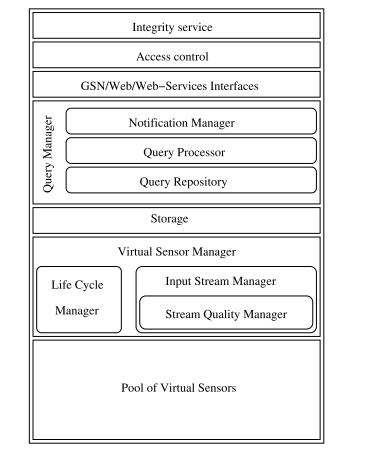
\includegraphics[width=0.8\textwidth]{Chap2/figures/gsn_arch.png}
		\caption{GSN Architecture \cite{F2006}}
		\label{bg:fig:gsn}
		\end{figure}

Figure \ref{bg:fig:gsn} outlines the architecture of GSN, showing that the virtual sensors are stored on a central node and their inputs are managed and stored. GSN also comes bundled with a web interface to show all active sensors and their most recent recordings, as well as the implementation of web services to access the data outside of the interface.

Data from virtual sensors pass through the virtual sensor manager to the storage layer. Once the data has been stored, the query manager is invoked and queries are loaded from the repository and executed by the manager. The results of the queries are then handled by the notification manager and also made available to the web interface. Notifications can be extended to support many different forms of communication, such as SMS, email or web services.

Virtual sensors do not natively support all hardware, although new virtual sensors can be described using XML, and there may be a need to implement an entirely new virtual sensor. In this case, technical knowledge is required, and new sensors can be implemented through use of the Java programming language. This provides more control over the use of XML and allows users to specify how sensed data is stored in a database, use external libraries to receive proprietary data, specify processing workflows before the data is stored or implement new notification methods for the users of the network.

To show the simplicity of a basic virtual sensor, \cite{Aberer2007} describes a temperature sensor that we reproduce here in Listing \ref{bg:lst:gsn:vsensor}. The file is human-readable and does not require specialist knowledge when compared with programming languages, with tags that have self-explanatory names. In this example, the output structure shows that only a temperature reading is received and that the data should be stored permanently. The stream source specifies the content of the stream and the query details the standard query that should be used to extract data from GSN.

\begin{lstlisting}[caption={Example Virtual Sensor},label={bg:lst:gsn:vsensor}]
<life-cycle pool-size="10" />
<output-structure> 
	<field name="TEMPERATURE" type="integer"/> 
</output-structure>
<storage permanent-storage="true" size="10s" /> 
<input-stream name="dummy" rate="100" > 
<stream-source alias="src1" sampling-rate="1" storage-size="1h">
<address wrapper="remote"> <predicate key="type" val="temperature" /> <predicate key="location" val="bc143" /> </address> 
<query>select avg(temperature) from WRAPPER</query>
</stream-source>
<query>select * from src1</query> 
</input-stream>

\end{lstlisting}

The modularity and flexibility of GSN makes it different to existing middlewares as it has not been designed for any specific hardware and modules of the middleware can be replaced, such as the database. 



	\subsubsection{FACTS}
		One such example is the FACTS middleware, an approach that uses a fact repository to coordinate nodes. Rules can then be implemented to process sensed data and fired when certain conditions are met \cite{Terfloth2006}. More traditional sensor middlewares control the network and manage sensed data but this rule based approach allows for more flexibility, where rules can control the transmissions and process the data upon receipt.

		\begin{figure}[h]
		\centering
		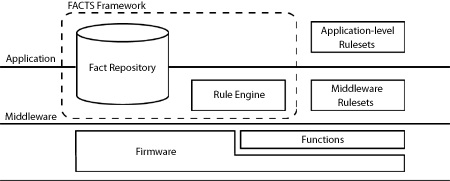
\includegraphics[width=0.8\textwidth]{Chap2/figures/facts_architecture}
		\caption{FACTS Architecturei \cite{Terfloth2006}}
		\label{bg:fig:facts}
		\end{figure}

		Figure \ref{bg:fig:facts} shows the FACTS architecture, with the middleware holding the rulesets and a dstributed fact repository. Data within the network is stored as facts, providing a standard data format throughout the network and hardware abstraction. When new facts are received, ususally because of new sensing data, the rule engine checks to determine whether any rules should be fired. The ruleset definition language (RDL) is used here and each ruleset contains a group of relevant rules. Each rule is given a priority so that, if more than one rule is triggered by a fact, then the higher priority rules are fired first.

		Listing \ref{bg:facts:rule} shows a FACTS rule, written in Haskell, that determines which geegraphic areas are covered by nodes. The name of each rule has no prefix, statements are prefixed with `->' and conditions are prefixed with `<-'. The \textit{sendRange} rule runs after a timer expires and removes that timer. Lines 4 to 12 set a \textit{rangeFact} fact that contains the range it expects to be able to cover. The rest of the rule sends the fact to all nodes within range and sets a new fact to show that it has sent its range information. 

		The \textit(xyMinCovered) is a simplified rule that, upon receipt of range information from neighbouring nodes, checks whether the range of the neighbouring node overlaps with its own range and the final \textit{determineCoverage} rule then stores that coverage information in a fact as knowledge of whether or not it is the only node to cover a particular geographic region. This can then be used to inform future routing and sleeping decisions.

		\begin{lstlisting}[caption={Coverage Algorithm in FACTS Rules}, label={bg:facts:rule}]
 sendRange
 <- Exists Timer.expiredSlot
 -> Retract Timer.expiredSlot 
 -> Define "rangeFact"
 -> Set ("rangeFact" "xMin")
	(posXSlot - System.txRadiusSlot)
-> Set ("rangeFact" "xMax") 
	(posXSlot + System.txRadiusSlot)
-> Set ("rangeFact" "yMin")
	(posYSlot - System.txRadiusSlot)
-> Set ("rangeFact" "yMax")
	(posYSlot + System.txRadiusSlot)
-> Send 0 System.txPowerSlot 
	("rangeFact" [(("rangeFact" "owner")
	== nodeIDSlot)])
-> Define "rangeSendFact"

xyMinCovered
<- Exists "rangeSendFact"
<- Eval ((posXSlot - System.txRadiusSlot)
	< ("rangeFact" "xMin"))
<- Eval ((posYSlot - System.txRadiusSlot)
	< ("rangeFact" "yMin"))
-> Define "xyMinCoveredFact" 

determineCoverage
<- Exists xyMinCoveredFact"
-> Define "coveredFact
		\end{lstlisting}

		While FACTS itself does not utilise any local knowledge, the repository is used as a source for all previously sensed data and would be an excellent source of knowledge to assist with the classification of future readings. Also, the ability to add new rulesets, without technical knowledge of the hardware of each node means that users of the network have the ability to add knowledge in the form of less technical, high-level rules.

	\subsubsection{ITA Sensor Fabric}
	The ITA Sensor Fabric is collaboration project between IBM, the US Army and the UK MoD. Sensor Fabric, or Fabric, is a two-way messaging bus and set of middleware services connecting network assets to each other and users \cite{Wright2009b}.

The core difference between the Fabric middleware and others is that not every node is sensing all of the time, sensor nodes are tasked when there is a requirement and they stop as soon as that task has been fulfilled. Similar to sinks in a traditional WSN, Fabric utilises Fabric nodes, which run the following three pieces of software:
\begin{enumerate}
	\item Message Broker - Provides the communication infrastructure.
	\item Fabric Registry - Holds information about the current deployment, such as all nodes deployed, all assets, routing information and tasks. Deployed in the form of a database.
	\item Fabric Manager - The main service on the node to track the status of connected sensors, establish communication channels, provide a container for processing, plug-ins and to extends the capabilities of the Fabric.
\end{enumerate}

Fabric runs on a Publish/Subscribe model, a sensing requirement is sent to a messaging broker as a subscription and this is distributed through all Fabric nodes and, thus, all sensor nodes. Sensor nodes then publish their data and the relevant data is sent to all applications that have subscribed to the data. 

The plugin structure of Fabric makes it stand out from existing middlewares, allowing its functionality to be extended through web interfaces.

Because Fabric has been developed for military purposes that cross countries, policy enforcement has been implemented to restrict access to the granularity of sensed data but these access levels do not simply apply to a military context. Using our motivating scenario, researchers and professors should see animal images whereas the Sabah Wildlife Department should see images of hunters and people in the forest.


\section{Biodiversity and Environmental Monitoring Sensor Networks} \label{bg:bsn}
	In this section we will cover existing WSNs that are related to our motivating scenario or, more specifically, biodiversity focussed WSNs that have been deployed to monitor wildlife and/or the environment. WSNs for habitat, and wildlife, monitoring are especially important because these are areas that often need to be untouched by humans. Areas with high human disturbance can influence the abundance of species and some habitats, i.e. underground burrows, may be impossible to monitor without destruction. 
	
	One of the most well known WSNs to monitor habitat is the network deployed on Great Duck Island, an island off the coast of Maine, USA. A hierarchical network of 32 nodes was deployed to monitor a bird, known as the leach’s storm petrel \cite{Mainwaring2002}. This network used a clustering approach for groups of nodes to send data to a gateway node, which would then route it back to the base station. The base station, located a few kilometres away on the island, has internet access and uploads the data to allow users to browse and process the data.

	A multihop approach was used here as they found that, for sufficient coverage, single hop connectivity would not cover all of the island. Acrylic enclosures were developed to ensure the nodes were weatherproofed for the conditions of the island, while maintaining the functionality of each sensor and not impeding transmission range. While the nodes, their casing and their sensors have been designed specifically for the deployment on Great Duck Island, the success of the network, running for 123 days in the early stages of WSN research \cite{Szewczyk2004c}, shows that this approach can be used elsewhere with similar effects; allowing hard to monitor and/or inaccessible areas to be continuously monitored.

	On a smaller scale, INternet-Sensor InteGration for HabitaT monitoring (INSIGHT) is a single-hop WSN that allows remote access for data and reconfiguring of nodes \cite{Demirbas}. Using off the shelf hardware, their findings show that their nodes could survive for 160 days on a single battery, supporting their claim that a single hop network allows for a longer network lifetime. 
	
	The key feature of this network is the ability for humans to remotely set reporting thresholds for sensor nodes. This means a user can prolong the lifetime of nodes by limiting the threshold they report on, as well as the fact that these thresholds are a way for users to add knowledge, albeit primitive, into a network.

	While there is research on cameras used to monitor animals \cite{Kays2009, Ahumada2011a}, these ‘networks’ are generally cameras deployed with their memory cards manually retrieved and processed. In recent years, however, the use of wireless technologies and image-based WSNs has increased, \cite{Garcia-Sanchez2010b} uses wireless cameras to monitor the movement of animals between roads. Using commercial hardware and controlled sleep scheduling, this solution employs the use of nodes to detect movement and wake up more power-hungry camera nodes. While the nodes are wireless, the distance of the network from civilisation means that the data does still need to be collected manually and uploaded to a computer.

	Due to the advent of smartphones and tablets, as well as the improvements in 3G technology, projects taking advantage of more modern technologies have grown in popularity. Using 3G enabled cameras, \cite{ZSL} have deployed a number of devices in locations all over the world, such as: Kenya, Indonesia and the USA. The images captured are transmitted to a server and a website allows the general public to not only see the images in near real-time, but to classify the images as well. This crowdsourcing of collective knowledge lets people, that may not have domain knowledge, vote on an image and those votes are used to make classification easier.

	Over the past fifteen years, WSNs have grown from a concept to a real solution for monitoring the habitats, movements and eating habits of wildlife all over the world. Whether it is using GPS collars to monitor the movement of cattle \cite{Guo2006}, monitoring animal habitats on a remote island or using cameras to capture the animals themselves, the popularity of these networks has grown considerably and advances in technology have allowed these networks to be deployed in places that humans cannot access with ease.
	
		There are a number of situations where we may want to record data in an environment that is not safe for humans, such as a volcano \cite{Werner-Allen2006}, or that may be difficult for electronics to survive. In these cases, special considerations must be made during the design and deployment of the WSN, in order to ensure maximum  network lifetime with reliable readings.
	\subsubsection{GLACSWEB}
	Glacsweb is a sensor network to monitor the rate that which glaciers are melting. Deployed in Norway, specially designed sensors have been drilled into glaciers to monitor pressure, temperature, orientation and strain. Due to the high pressure and exposure to moisture, a polyester casing was used so that, once bonded, the node inside would be protected from its environment, but also preventing it from being recoverable.
	\subsubsection{Reventador}
	Volcano Reventador is in northern Ecuador and a WSN has been deployed on there to monitor eruptions. Similar to Glacsweb, weatherproof enclosures were used to prevent ash and moisture from breaking the sensors and long-range external antenna mounted to a pole was used to achieve communications over large distances when wireless communications have proven to be difficult \cite{Werner-Allen2006}.
	\subsubsection{Rainforest}
	There have been many studies on how the rainforest affects the range and quality of wireless links \cite{Figueiredo2009, Wark2008, Rahman2008}. In \cite{Figueiredo2009}, the humidity was shown to reduce 802.11 range by up to 78\% and \cite{Wark2008} explains that periods of rainfall reduce the link quality up to 100\% in some cases, resulting in the loss of a hop and this could prevent data from reaching the endpoint.


This section highlights the difficulties of deploying a WSN in harsh environments. Environments vary from freezing glaciers to humid rainforests to dry, scorching deserts and the areas the sensors are placed in cannot disturb their surroundings, be too conspicuous or require regular human attention that would disturb the area. 

\section{Local and Global Knowledge} \label{bg:lgk}
	The environment of a sensor network is rich and varied and we believe that knowledge of this environment and patterns in the data sensed can be used to inform the network on decisions surrounding the transmission and processing of newly sensed data. As our research began, we simply called this knowledge but, as our work continued, it became apparent that it could be catgorised further.

While we believe that we are the first to use the concept of local and global knowledge within the wireless sensor network domain, the terms have been around for many years. In 1999, a book that referred to local knowledge as \textit{indigenous knowledge} defined local knowledge as ‘systematic information that remains in the informal sector, usually unwritten and preserved in oral traditions rather than text’ \cite{LadislausM.Semali}. 

Over the past twenty years, local knowledge has been used in various contexts, from researching lending and the credit market \cite{Stiglitz1990} to extracting local knowledge from natives to improve farming techniques \cite{DEWALT}. This research, as well as work that will be covered later, showed us that there are two kinds of knowledge: global and local. 

It was from agriculture research that we were able to refine our definition of local knowledge, \cite{Joshi2001} defines local knowledge as ‘knowledge that farmers have derived locally through experience and experimentation’. They also say that indigenous knowledge is different in that it is culturally specific. From this definition, as well as our work with our motivating scenario, we were able to generalise the definition and expand upon it.

We now define local knowledge as \textit{knowledge of an area, held by a domain expert, that has been gained through experience or experimentation}. This then means that global knowledge is \textit{knowledge of an area that can be accessed by anyone, without the need to visit the area directly}. The weather of a region is global knowledge because it can be found through a variety of media, whereas the saturation levels of the soil in a field would be local knowledge as it would require experimentation to gain that knowledge. Local knowledge could become global if it was readily available but some of these data are held in tribes of people without Internet access.

Using these definitions, we believe that \textbf{encoding local and global knowledge onto sensors can inform routing decisions to make better use of the bandwidth in resource-constrained WSNs by sending data that the node believes to be important first, rather than chronologically}. Patterns in the data, and knowledge of the environment surrounding a node, can allow a node to infer what the data may be valuable, automate the processing of adding context to the sensed data, learn from previously sensed data and utilise global knowledge of ongoing projects within the network to determine what data is thought to be of a higher priority.

\section{Relevant Existing Networks} \label{bg:rsn}
	In this section, we discuss existing networks that are related to our research question and/or motivating scenario. While most of the existing networks relevant to Danau Girang have already been covered in Section \ref{bg:bsn}, there are some WSNs that are not directly related to biodiversity but have been deployed in harsh conditions or involve interdisciplinary collaboration. Interdisciplinary networks are of particular interest because they include the crossover of specialist knowledge from two, or more, domains. For example, biodiversity networks combine computer networking and software development and bioscience while medical networks combine medical knowledge. This means that the networks must be developed with the operation of users that may not possess the same specialist knowledge in mind and, thus, need to be more generally accessible. These examples prove invaluable when designing our own WSN architecture as some middleware and hardware solutions have been created with ease of use as a priority and do not require technical knowledge, allowing them to be used with little training.

\subsection{Context-Awareness}
	While standard WSNs have been prevalent for many decades, new research on the Internet of Things \cite{Atzori2010} has brought about interest in context-aware sensing, in some cases this is for small wearable devices to track fitness but the applications are much broader. Here we will look at WSNs that use context to make informed routing decisions, save power, or prioritise the transmission of data. We consider context-aware sensors the step before a network making use of local and global knowledge and the uses of knowledge in these scenarios will only enhance the data further.

	\subsubsection{Health}
		Health monitoring is one of the more obvious choices for context awareness as classifying readings can often help determine the health of someone, rather than their self-reports. AlarmNet is a WSN that uses context to provide long-term health monitoring for people in assisted-living environments \cite{Wood}.
	
AlarmNet employs context-awareness to learn about the activity levels of the patient and uses that knowledge to determine when changes in the readings may mean that the patient is at risk. Once the AlarmNet system has completed its learning period, deviations, from what it has recorded as the normal activities for the patient, are sent to nurses and doctors, with the idea that this information can assist with a diagnosis.

As some nodes in the system will be battery powered, AlarmNet also employs a subsystem, called the Context-Aware Power Management System (CAPM), to control the power consumption of a device based on the recorded activities of the patient. The system uses policies, based on the context, to save power for all nodes in the system. For example, the system could put mains-powered nodes into a low-power state and disable all nodes outside of the bedroom when it detects that the patient has gone to sleep.

This use of context has not only shown that it can assist with the lifetime of a network, but it can also provide valuable insight into sensed data to provide data enriched with semantics.

	\subsubsection{Wearable Devices}
As wearable devices, such as the Fitbit and the Pebble smartwatch, are increasing in popularity, context-awareness is a useful tool to differentiate between the many activities that a person can undertake. The MObile PErsonal Trainer system (MOPET) is a wearable fitness devices that uses context to record data on jogging and fitness exercises \cite{Buttussi2008}. 

While the project is five years old now, it is one of the earliest proof-of-concept devices created and shows how simple rules applied to sensor readings can be used to apply context. For example, the device consists of a GPS sensor and, when active, it is constantly recording positions. Using pairs of points, it is able to calculate the speed and, if the speed is consistent with jogging, then it records a running exercise.

Fitness is not the only purpose for wearable computing, the eWatch is an early design for a \textit{smartwatch} that uses a microphone and light sensor to record the locations that the user visits, storing previous recordings in flash memory and matching them with current recordings \cite{Maurer}.

	% \subsubsection{UNETS}
	% 	*UNETS is tiered and context aware

\section{Summary}
	In this chapter we have explored the components that make a WSN, as well as some existing deployments that are relevant to our motivating scenario. Sensor middleware have come a long way in the past decade and increased capabilities for sensor nodes have allowed for more intense processing to be carried out before any data is seen by a human. Context is now used on sensor nodes to infer the activity they are undertaking or even to determine when it should wake to sample. 

Local knowledge is not a new concept and it has been used for many years to extract information from indigenous people and in industry to adapt their processes to a local area, such as farming. However, we believe that our work is the first to apply local knowledge in the context of WSNs. Context-aware sensor networks have gone some way to support out hypothesis that some knowledge can increase the functionality of a network and enhance the quality of the sensed data, but we believe that the addition of LK and GK will only increase this functionality further.

The two primary components of a WSN that could be injected with local knowledge is the middleware and the routing protocol, each providing different benefits. Existing work has shown middleware that uses context-awareness can use that to make global changes to the network \ref{bg:sm}, such as power management, whereas routing protocols affect the data that is sampled and sent to the endpoint(s) of the network, such as adaptive thresholds.

One issue in proving this hypothesis is the deployment of a network that utilises local knowledge. The deployment environment of our motivating scenario is not only interdisciplinary, it is in a region that is humid, dynamic and dense. Existing research has shown that the deployment of a WSN in these considerations means that range will be greatly reduced \cite{Figueiredo2009} and changes in humidity can prevent communication altogether, as well as moisture affecting the hardware itself.
To deploy a network, hardware must be adapted and the right medium must be chosen in order to maximise link quality and minimise dropped connections.

In Chapter 3, we describe how we used this research, along with our own findings, to choose suitable hardware for our network. As well as this, we used the results from previous rainforest range tests in the literature, to design  experiments that would aid us in choosing, and verifying, our choice of tranmsission medium.

